\documentclass{article}
\usepackage[left=3cm,right=3cm,top=2cm,bottom=2cm]{geometry} 
\usepackage[spanish]{babel}
\usepackage[doument]{ragged2e}
\usepackage{graphicx}
\usepackage{float}
\usepackage{amsmath}
\selectlanguage{spanish}
\usepackage[utf8]{inputenc}
\setlength{\parindent}{0mm}
\usepackage{listings}

\begin{document}

\lstset{language=C++}
\lstset{numbers=left}

\title{Práctica 1}
\author{Emilio José Hoyo \\ Stefan Parvanov}
\date{\today}
\maketitle

\section{Ejercicio 1 : Ordenación de la burbuja}
El siguiente código realiza la ordenación mediante el algoritmo de la burbuja:
\begin{lstlisting}
      void ordenar(int *v, int n) {
        for (int i=0; i<n-1; i++)
          for (int j=0; j<n-i-1; j++)
            if (v[j]>v[j+1]) {
              int aux = v[j];
              v[j] = v[j+1];
              v[j+1] = aux;
		} 
      }
\end{lstlisting}

Calcule la eficiencia teórica de este algoritmo. A continuación replique el experimento que se ha hecho antes (búsqueda lineal) con este nuevo código. Debe:
\begin{itemize}
	\item Crear un fichero ordenacion.cpp con el programa completo para realizar una ejecución del algoritmo.
	\item Crear un script ejecuciones\_ordenacion.csh en C-Shell que permite ejecutar varias veces el programa anterior y generar un fichero con los datos obtenidos.
	\item Usar gnuplot para dibujar los datos obtenidos en el apartado previo
\end{itemize}
Los datos deben contener xtiempos de ejecución para tamaños del vector 100, 600, 1100, ...,30000. \\
Pruebe a dibujar superpuestas la función con la eficiencia teórica y la empírica. ¿Qué sucede? 
\clearpage

Empezamos calculando la eficiencia te\`orica:
\begin{itemize}
	\item Linea 2: \\ Al principio del bucle siempre tendremos 3 OE :la asignaci\`on i=0\ ; la resta  n-1 y la comparaci\`on. Al final de cada iteraci\`o tambi\`en se ejecuta 1 OE (el incremento del contador). El bucle ejecuta n-2 veces su cuerpo.
	\item Linea 3: \\ Al igual que antes tenemos las 3 OE iniciales y 1 OE en cada iteraci\`on. El bucle se ejecuta n-i-2 veces.
	\item Linea 4: \\ Se ejecutan 4 OE : 2 accesos a memoria, una operaci\`on aritm\`etica y una comparaci\`on.
	\item Lineas 5, 6, y 7 \\  Se ejecutan 9 OE.
\end{itemize}
	Obtenemos el siguiente tiempo de ejecuci\`on: 
	\begin{equation}
		T(n)= 3 + \sum\limits_{i=1}^{n-1}{3+1+3+\sum\limits_{j=1}^{n-i-1}{3+1+4+9}}
	\end{equation}
	Mediante gnuplot
	
\clearpage
\section{Ejercicio 2 : Ajuste en la ordenación de la burbuja}
Replique el experimento de ajuste por regresión a los resultados obtenidos en el ejercicio 1 que calculaba la eficiencia del algoritmo de ordenación de la burbuja. Para ello considere que f(x) es de la forma ax2+bx+c

\clearpage
\section{Ejercicio 3 : Problemas de precisión}
Junto con este guión se le ha suministrado un fichero ejercicio\_desc.cpp. En él se ha implementado un algoritmo. Se pide que:
\begin{itemize}
	\item Explique qué hace este algoritmo.
	\item Calcule su eficiencia teórica.
	\item Calcule su eficiencia empírica.
\end{itemize}
Si visualiza la eficiencia empírica debería notar algo anormal. Explíquelo y proponga una solución. Compruebe que su solución es correcta. Una vez resuelto el problema realice la regresioón para ajustar la curva teórica a la empírica.


\clearpage
\section{Ejercicio 4 :}
Retome el ejercicio de ordenación mediante el algoritmo de la burbuja. Debe modificar el
código que genera los datos de entrada para situarnos en dos escenarios diferentes:
\begin{itemize}
	\item El mejor caso posible. Para este algoritmo, si la entrada es un vector que ya está ordenado el tiempo de cómputo es menor ya que no tiene que intercambiar ningún elemento
	\item El peor caso posible. Si la entrada es un vector ordenado en orden inverso estaremos en la peor situación posible ya que en cada iteración del bucle interno hay que hacer un intercambio.
\end{itemize}
	Calcule la eficiencia empírica en ambos escenarios y compárela con el resultado del ejercicio 1.
\clearpage
\section{Ejercicio 5 : Dependencia de la implementacin}
Considere esta otra implementación del algoritmo de la burbuja:
\begin{lstlisting}
	void ordenar(int *v, int n) {
		bool cambio=true;
		for (int i=0; i<n-1 && cambio; i++) {
			cambio=false;
			for (int j=0; j<n-i-1; j++)
				if (v[j]>v[j+1]) {
					cambio=true;
					int aux = v[j];
					v[j] = v[j+1];
					v[j+1] = aux;
				}
		}
	}
\end{lstlisting}

En ella se ha introducido una variable que permite saber si, en una de las iteraciones del
bucle externo no se ha modificado el vector. Si esto ocurre significa que ya está ordenado
y no hay que continuar.
Considere ahora la situación del mejor caso posible en la que el vector de entrada ya está
ordenado. ¿Cuál sería la eficiencia teórica en ese mejor caso? Muestre la gráfica con la
eficiencia empírica y compruebe si se ajusta a la previsión.

Empecemos calculando la eficiencia teórica:
\begin{itemize}
	\item Línea 2: 1OE (asignación).
	\item Línea 3: 1OE (asignación) + 3OE (resta, comparación,
          operación \&\&) + 1OE (incremento).
	\item Línea 4: 1OE (asignación).
	\item Línea 5: 1OE (asignación) + 3OE (resta*2, comparación) + 1OE (incremento).
	\item Línea 6: 3OE (acceso al elemento [j] y [j+1], comparación).
	\item Línea 7: 1OE (asignación).
	\item Línea 8: 2OE (acceso al elemento [j], asignación).
	\item Línea 9: 3OE (acceso al elemento [j] y [j+1], asignación).
	\item Línea 10: 2OE (acceso al elemento [j+1], asignación).
\end{itemize}
Obtenemos el siguiente tiempo de ejecución en el mejor de los casos
(con el número de línea entre paréntesis):
\begin{align*}
  T(n)= 1OE(2) + 4OE&(3) + 1OE(4) + 4OE(5) + (( 3OE(6) + 1OE(5) +
  3OE(5) )*(n-1))\\& + 1OE(3) + 3OE(3) = 14+7n-7 = 7n+7
\end{align*}
La gráfica obtenida con gnuplot es la siguiente
\begin{figure}[H]
  \caption{Eficiencia en el mejor caso}
  \centering
  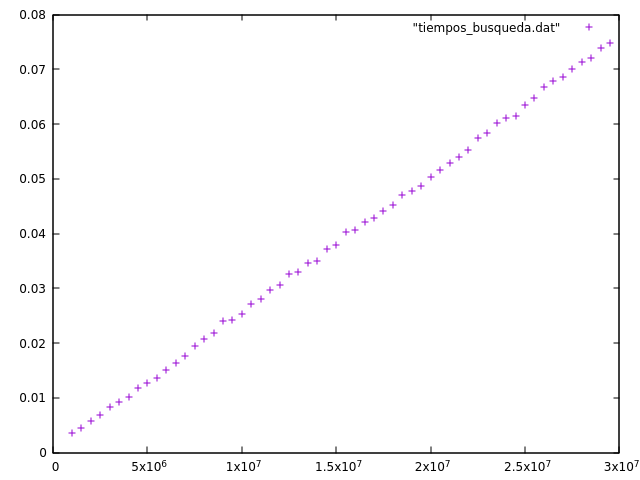
\includegraphics[width=0.8\textwidth]{ejer5/grafica.png}
\end{figure}
Como podemos ver si se ajuta a la teórica pues la mayoría de valores
de la gráfica se agrupan formando una recta.
\end{document}
